
\subsection{Репрезентативность (и сбалансированность?) корпуса, достоверность данных} \label{sect_corpus_representativeness}

Репрезентативность 
(не путать с представительностью)\footnote{Представительный корпус -- 
это корпус, обеспечивающий максимально широкое покрытие  
различных типов текстов и функциональных стилей~\cite{Sharov2004}.
} 
корпуса (текстовых примеров) 
эмпирически определяют тем, в какой степени эти примеры показывают 
вариативность исследуемого явления~\cite{Biber1993representativeness}. 
Из этого определения следует, что нельзя говорить об универсальной 
представительности корпуса, но можно говорить 
о степени репрезентативности корпуса при решении конкретной лингвистической задачи.

В работе~\cite{Belikov2013}
оценивается достоверность корпусных исследований. 
Часто исследователи подвержены соблазну распространить опыт, полученный на конкретном корпусе, 
на весь язык, что неправомерно~\cite{Belikov2013}.

Каковы границы применимости разрабатываемого Открытого корпуса вепсского и карельского языков? 
Для ответа на этот вопрос нужно определить, тексты каких жанров и в какой пропорции включены в корпус ВепКар. 
Объём корпуса ВепКар составляет соответственно 2~677 текстов и 960~553 слов в текстах\footnote{ Данные на 23 апреля 2020~г. Cм. подробнее 
\href{http://dictorpus.krc.karelia.ru/ru/stats/by\_corp}{http://dictorpus.krc.karelia.ru/ru/stats/by\_corp}.}.

На рисунках \ref{fig:text_distr_by_corpus} и \ref{fig:text_distr_by_genre} показано распределение текстов по подкорпусам и жанрам для вепсского языка и наречий карельского языка\footnote{ Данные на 23 апреля 2020~г. Cм. подробнее 
			\href{http://dictorpus.krc.karelia.ru/ru/corpus/corpus}{http://dictorpus.krc.karelia.ru/ru/corpus/corpus}.}.

\begin{figure}
    \centering
    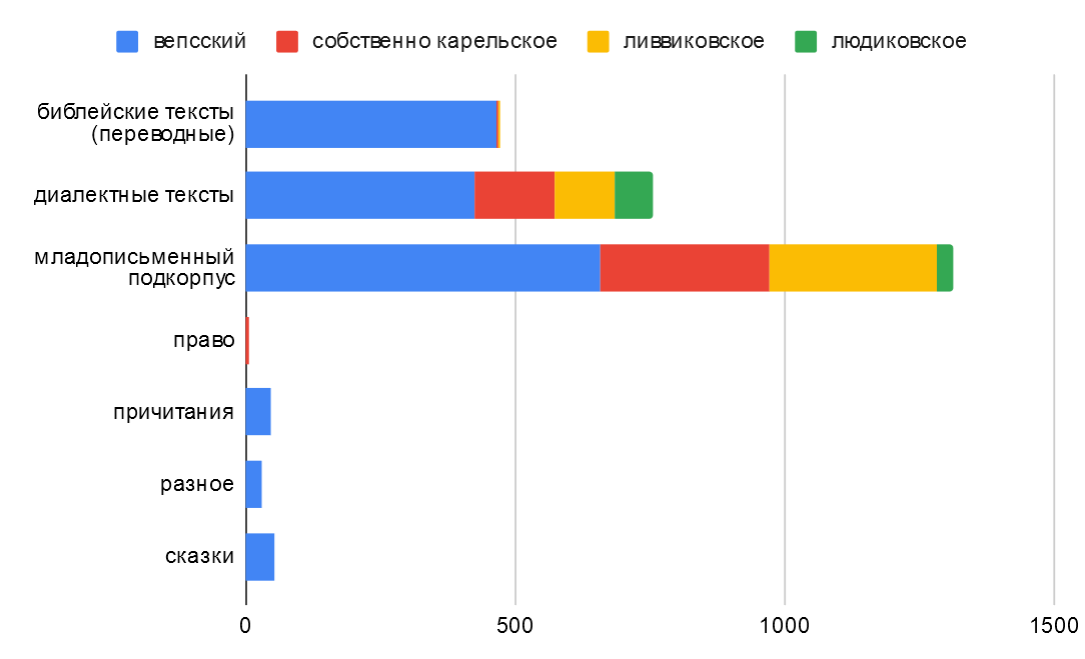
\includegraphics[width=1.0\textwidth,keepaspectratio=true]{text_distr_by_corpus.png}
    \caption{Распределение текстов по подкорпусам (вепсский язык и наречия карельского языка).}
    \label{fig:text_distr_by_corpus}
\end{figure}
%\bigskip

\begin{figure}
    \centering
    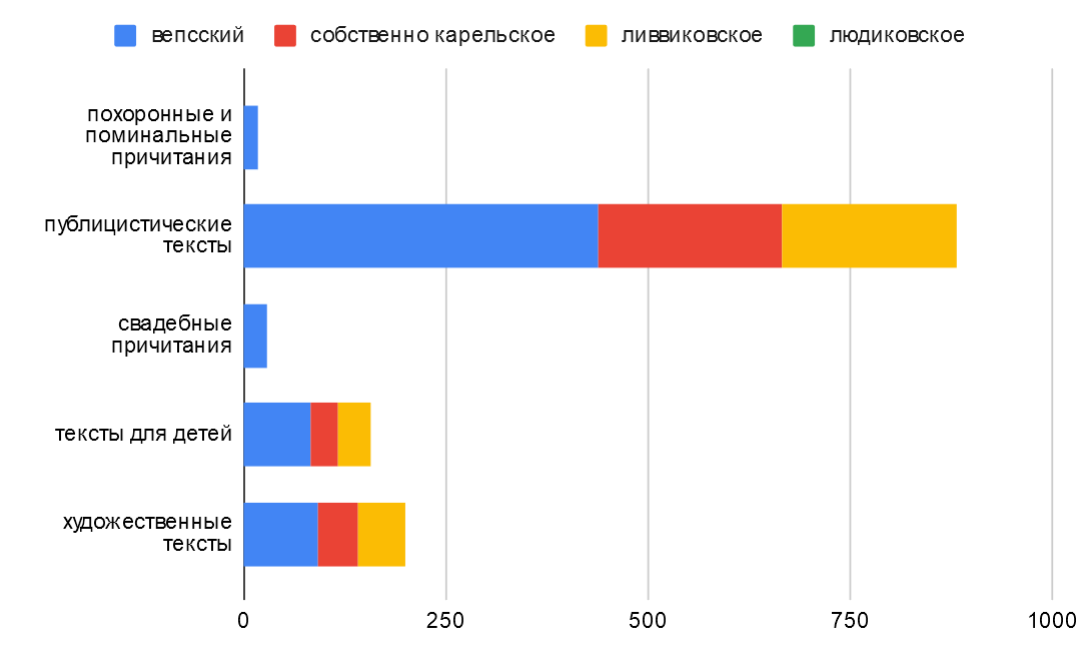
\includegraphics[width=1.0\textwidth,keepaspectratio=true]{text_distr_by_genre.png}
    \caption{Распределение текстов по жанрам (вепсский язык и наречия карельского языка).}
    \label{fig:text_distr_by_genre}
\end{figure}

Анализ временной динамики корпуса ВепКар показан на рисунке \ref{fig:text_distribution_by_date}. 2041 текстов (86,67\%) не имеют информации о дате записи.
\begin{figure}
    \centering
    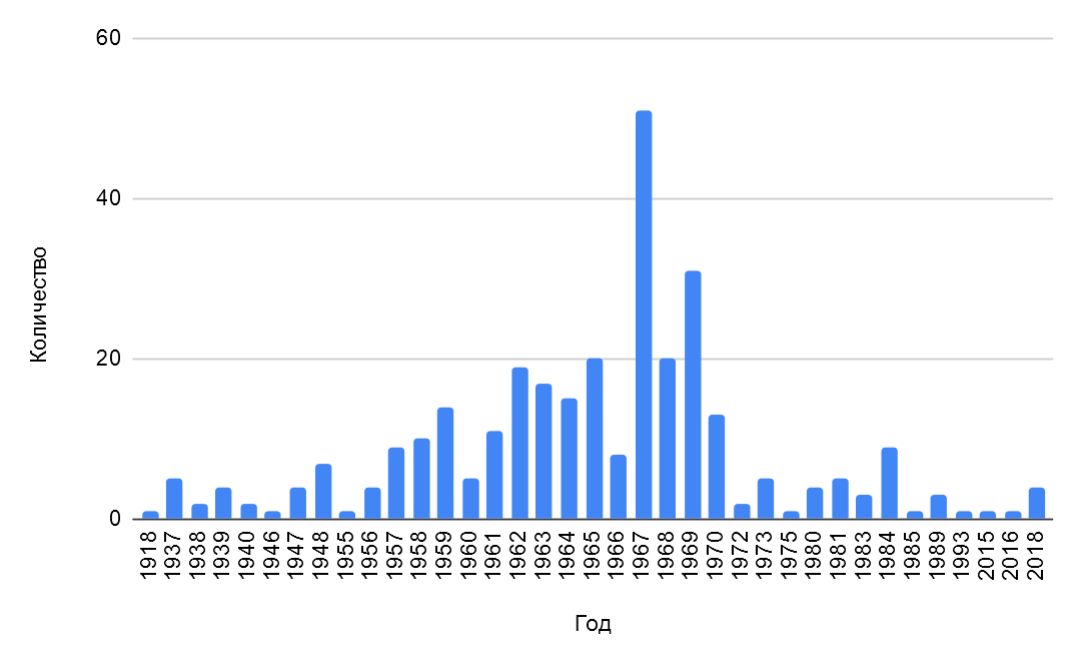
\includegraphics[width=1.0\textwidth,keepaspectratio=true]{text_distribution_by_date.png}
    \caption{Распределение числа текстов по годам.}
    \label{fig:text_distribution_by_date}
\end{figure}

Своевременно ли говорить о сбалансированности и представительности корпуса ВепКар? Вопрос остаётся открытым, нужны дополнительные исследования.
%Ответом может послужить информация о доле слов из словаря, употреблённых в текстах корпуса. 
\nata{TODO: Подсчитать долю / процент слов (для каждого из языков), которые встречаются в текстах. Процент + абсолютное число слов словаря в текстах.}
(Добавить эту статистику в корпус?)


